\chapter{Results}
\label{chapter:Results}

\begin{introduction}
    "The only source of knowledge is experience." - Albert Einstein
\end{introduction}

\section{Evolution of Software Development}

The software development process has undergone several important stages, each enhancing its functionality and usability. The figures below illustrate the application's progress, showcasing different phases of refinement as the project matured.

\subsection{Initial Stages: Basic Functionality and User Interaction}

The first figure (Figure \ref{fig:v1}) represents the early stages of development, where the primary focus was on creating a user-friendly interface for calculating average read depth and coverage metrics at diferent threshold from a BAM file for a Single Gene. In this version, the application prominently features a two-step process where the user selects a BED file releated to the gene to analyse and one or more BAM files. These files are then processed to calculate key metrics, which are displayed in the results table below. This simple design allowed for efficient user interaction but was somewhat limited in terms of flexibility and scope.

At this stage, the core challenge was to ensure that the software could handle large genomic files while presenting the results in a clear and intuitive format. The layout emphasizes simplicity, making it easier for users to navigate through the two-step process. However, as the project progressed, the need for more advanced features became evident.

\begin{figure}[H]
    \centering
    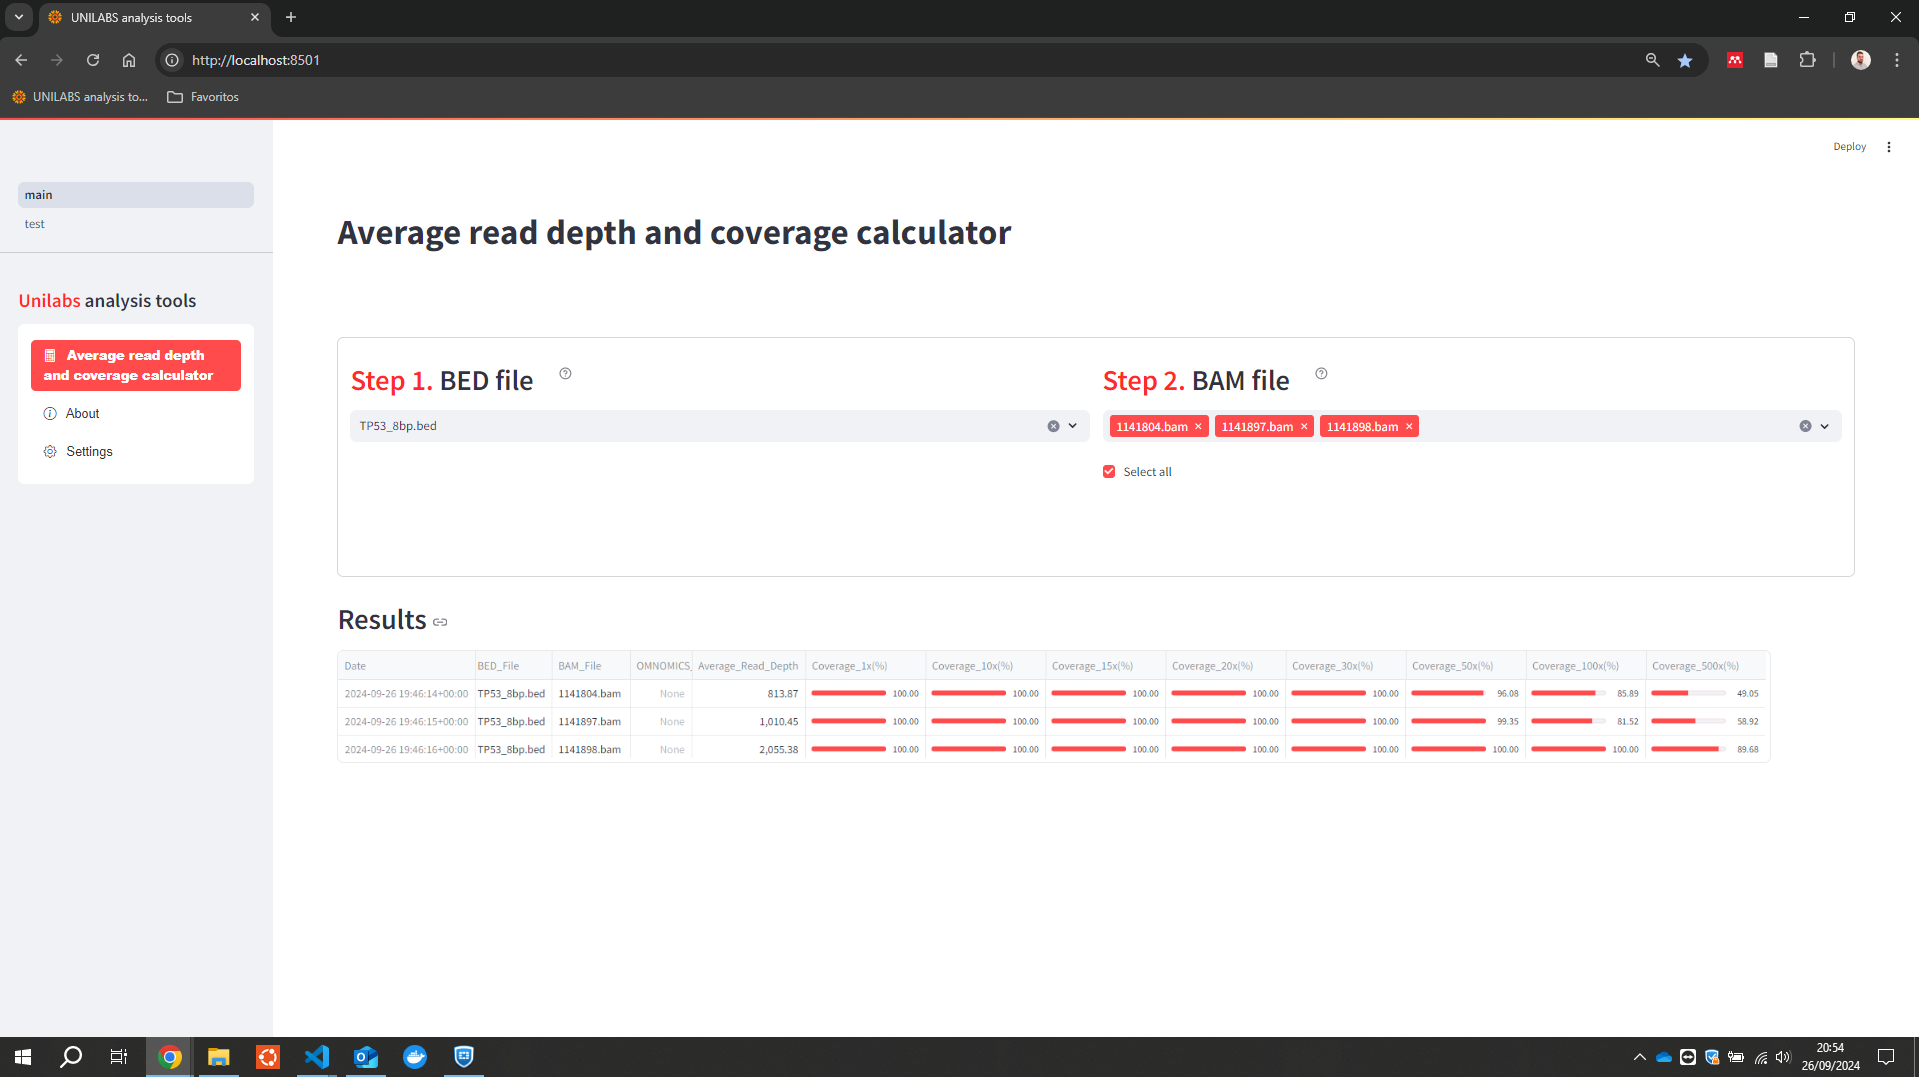
\includegraphics[width=1\textwidth]{figs/v1.png}
    \caption{First version of the GUI.} 
    \label{fig:v1}
\end{figure}

\subsection{Refinement: Introducing Flexibility and Multiple Analysis Modes}

In the second figure (Figure \ref{fig:v2}), the software has significantly evolved to include more detailed analysis options. The interface now presents multiple analysis types: \textit{Single Gene}, \textit{Gene Panel}, and \textit{Exome}, catering to different research needs. This flexibility represents a major shift from the earlier version, as it now allows users to select specific genome assemblies and regions of interest by using an universal BED file. Additionally, the results section has been split into tabs such as \textit{Overview} and \textit{Exon Details}, giving users the ability to drill down into the metrics for a the gene or explore exon-level coverage details. However, even though this last features were thinked to be used in this version, they only have been work fully in the last version of the software.

\begin{figure}[H]
    \centering
    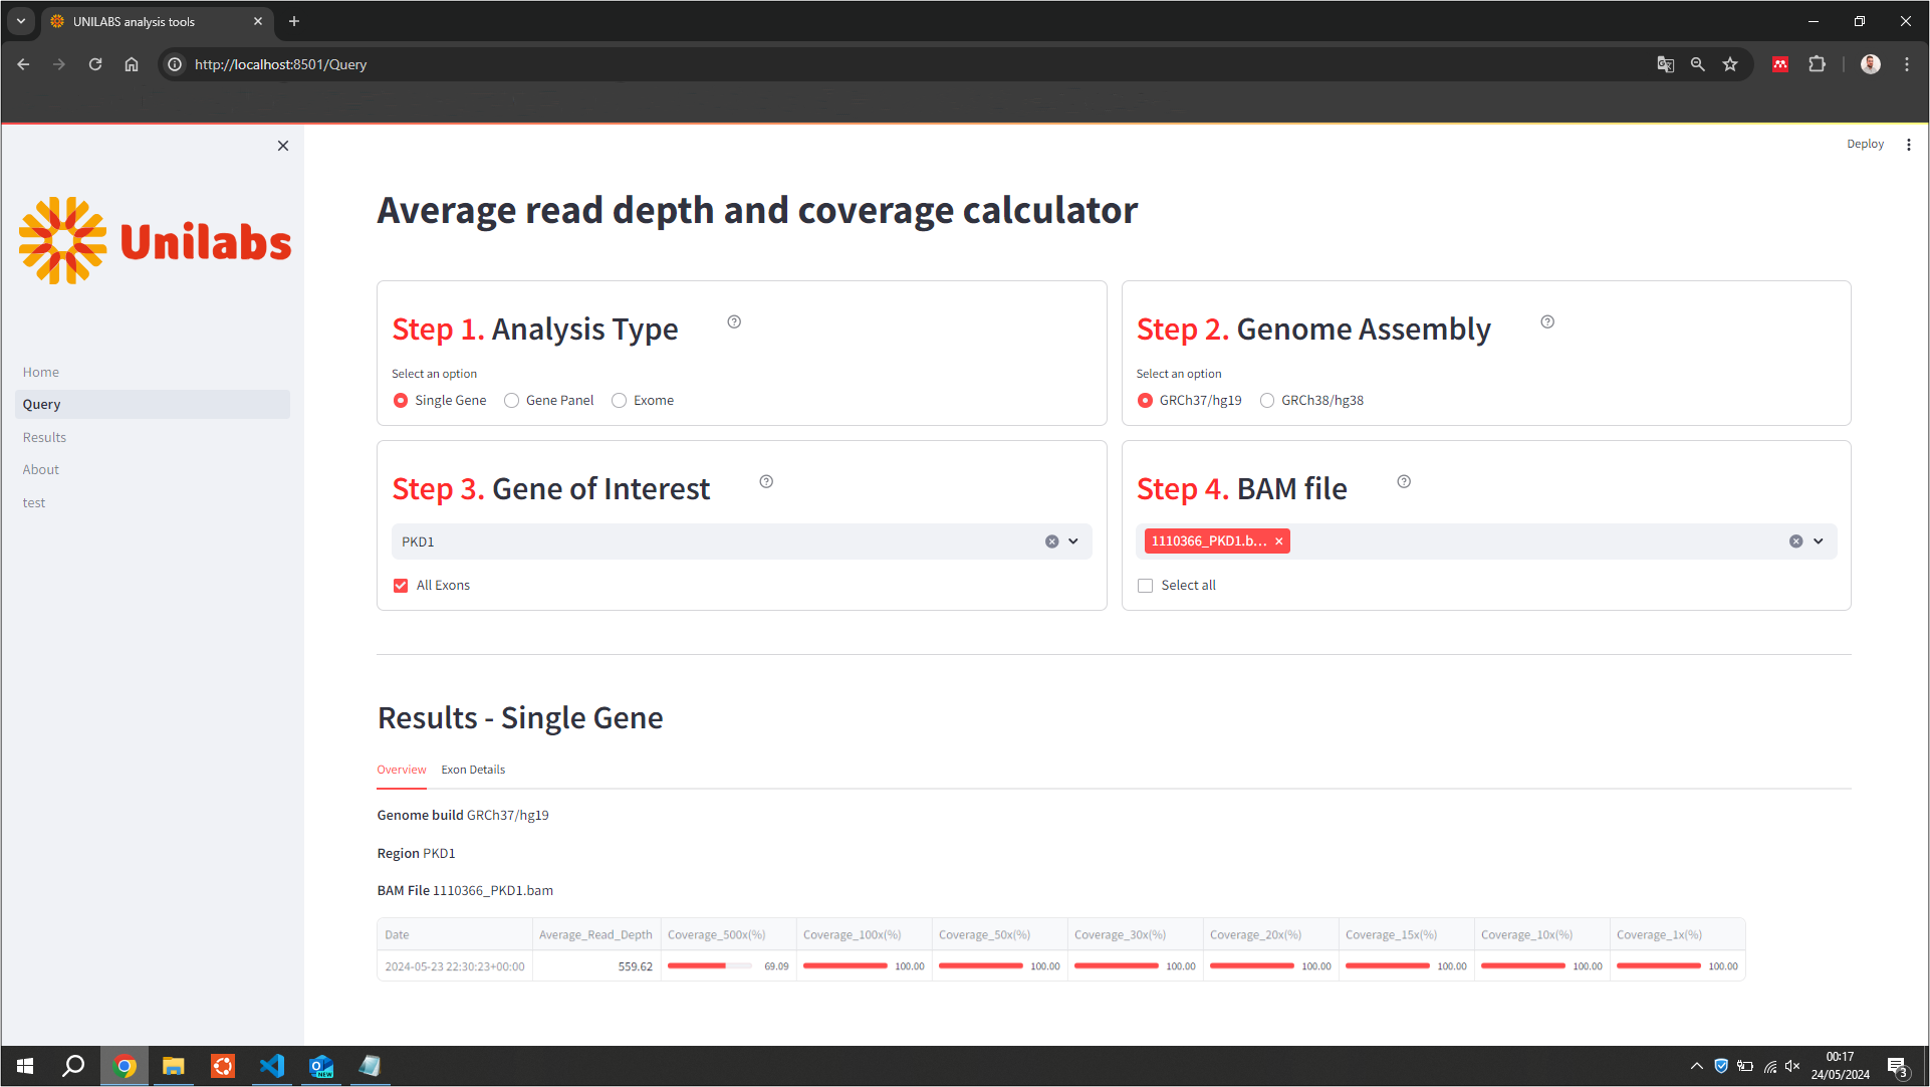
\includegraphics[width=1\textwidth]{figs/v2.png}
    \caption{Second version of the GUI.} 
    \label{fig:v2}
\end{figure}


The final version of the software is presented in the next section in detail with real-world data to showcase its full capabilities and effectiveness in genomic analysis. This final iteration represents the culmination of numerous improvements in both the user interface and the backend computational logic, making it a powerful tool for researchers.

\subsection{Overview of the Final Version}

The final version of the software maintains the core functionality established in earlier versions, such as calculating average read depth and coverage metrics from BED and BAM files. However, it has evolved to include more refined features, enhanced performance, and the ability to handle more complex datasets.

This section presents a detailed overview of the final version of the software using real-world genomic data, illustrating its capabilities in calculating read depth and coverage for genomic regions of interest. The images provided demonstrate the final interface and processing stages.

\subsubsection{\textbf{Login Interface}}

As seen in Figure \ref{fig:login}, the software begins with a user authentication process, offering a simple and clean login interface. This feature, although optional in the final deployment, ensures that access to sensitive data is controlled. Users must input their credentials, and upon successful authentication, they are granted access to the full range of analysis tools.

\begin{figure}[H]
    \centering
    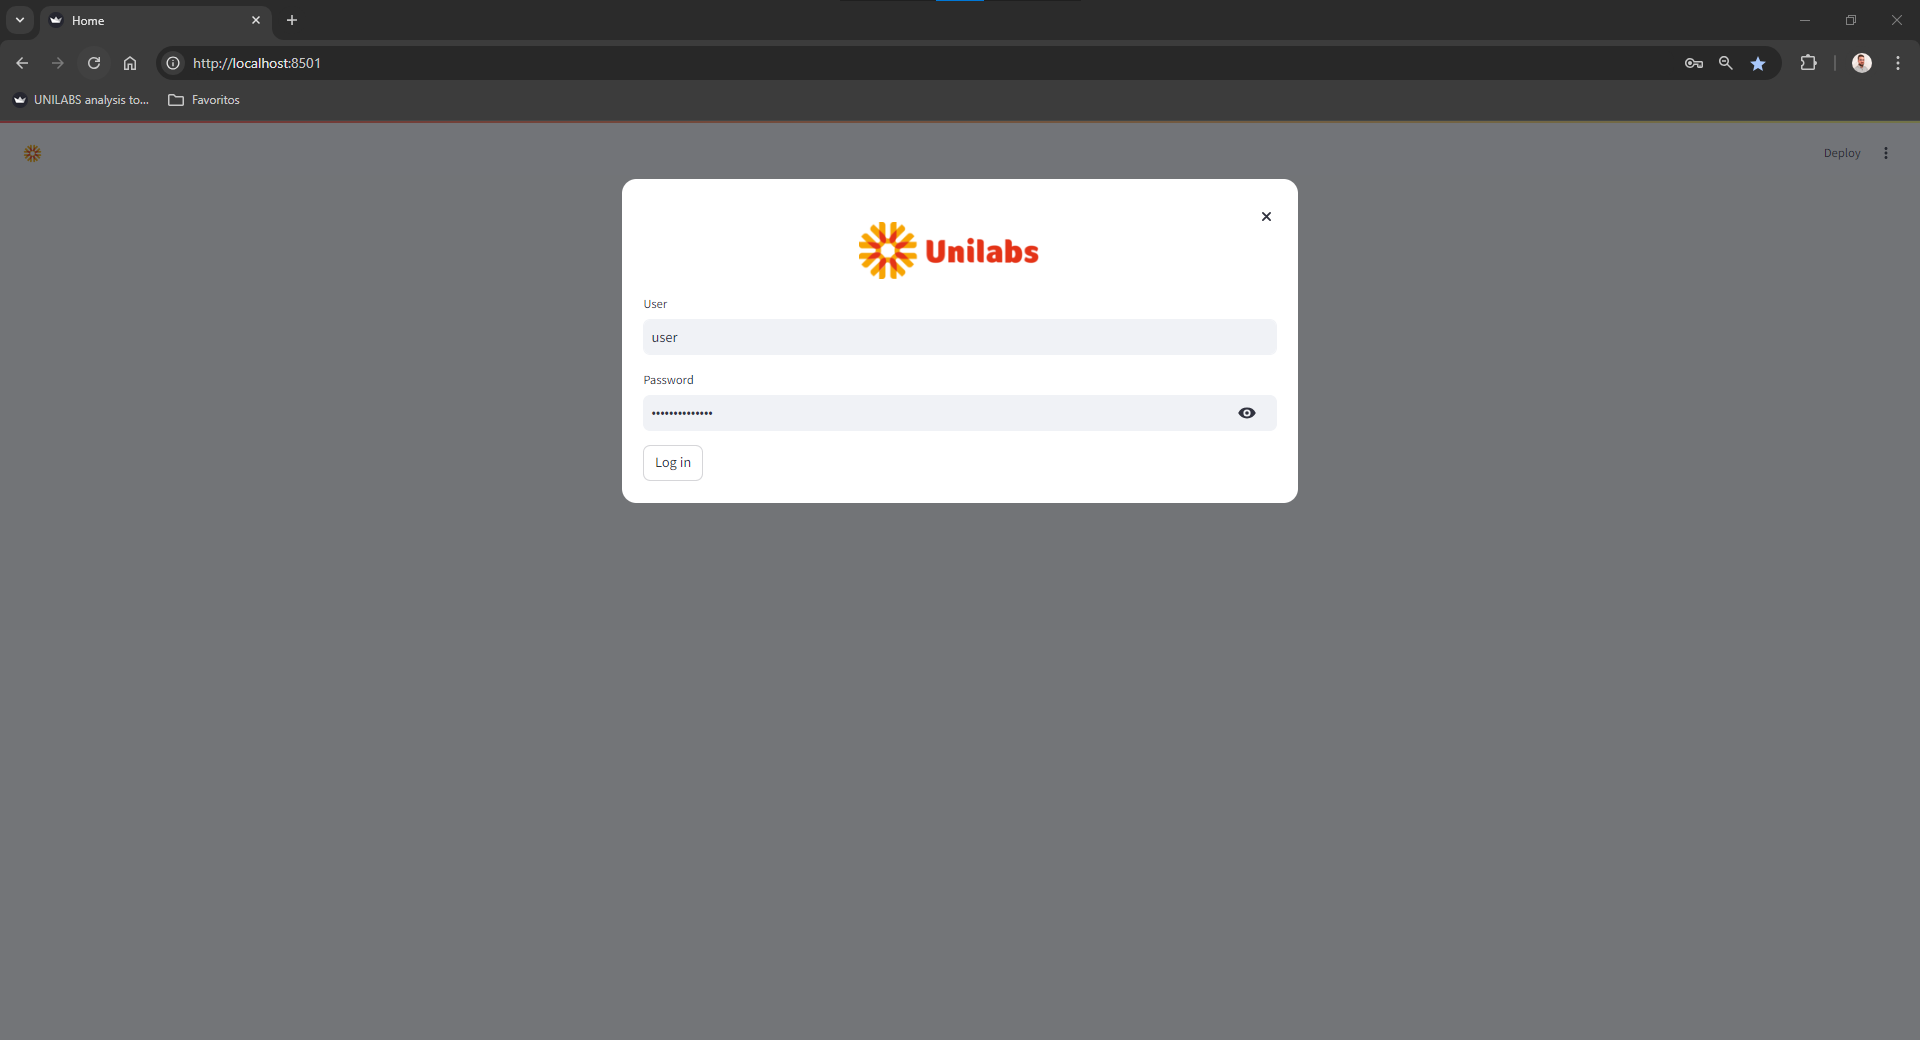
\includegraphics[width=\textwidth]{figs/v3.1.png}
    \caption{Login Interface for the Software}
    \label{fig:login}
\end{figure}

The next step of the process involves selecting the analysis type, as shown in Figure \ref{fig:single_gene}. Users can choose between three options: Single Gene, Gene Panel, and Exome. This selection determines the scope of the analysis and the subsequent steps in the workflow.


\subsubsection{\textbf{Single Gene Analysis}}

In this version, users can perform a single gene analysis by selecting the appropriate options for genome assembly and gene of interest. The software also provides the option to analyze all exons within the selected gene or focus on specific exons of interest. BAM/CRAM files containing the sequencing data are acessed and processed by samtools for detailed metrics.

\begin{figure}[H]
    \centering
    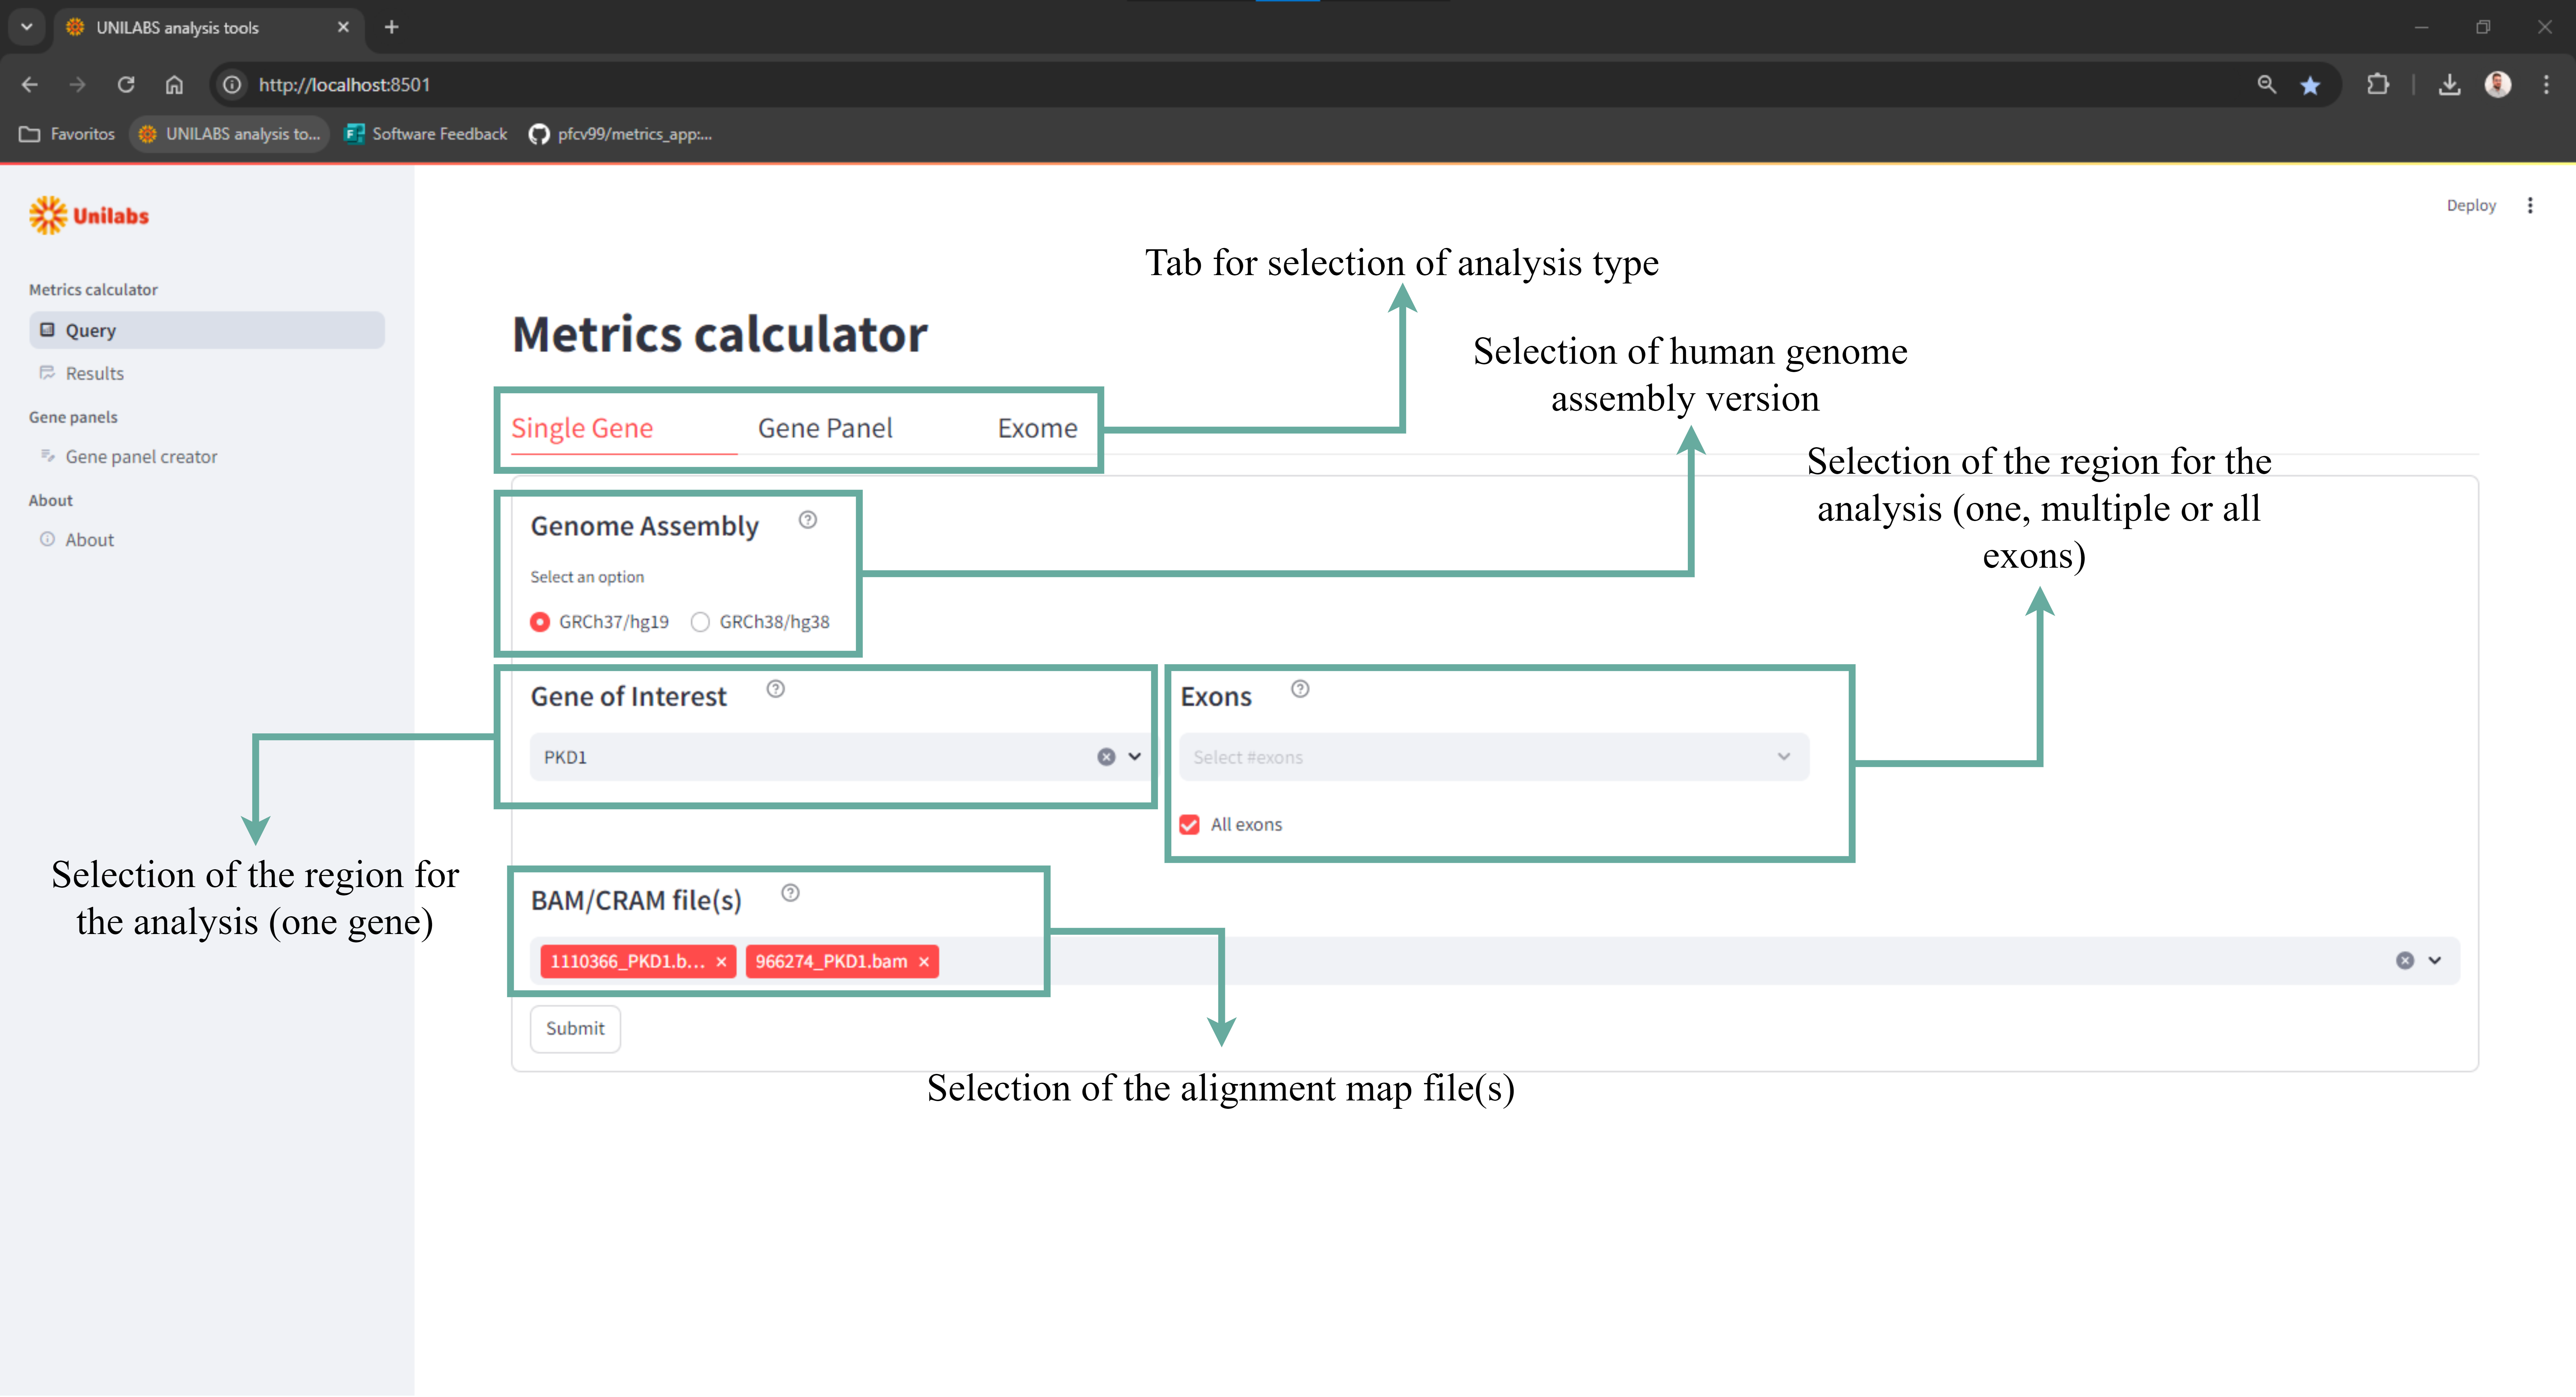
\includegraphics[width=\textwidth]{figs/v3.2.png}
    \caption{Single Gene Analysis Workflow}
    \label{fig:single_gene}
\end{figure}

\begin{itemize}
    \item \textbf{Results and Report Generation}

    Once the data is processed, users can access the results in the 'Results' tab, as seen in Figure~\ref{fig:results_loading}. The software compiles a detailed report that includes various metrics such as average read depth, breadth of coverage, and coverage percentages across different thresholds (e.g., 10x, 20x, 30x). This data is also available for download in a PDF format, ensuring users can retain a permanent copy of the analysis results.
    
    \begin{figure}[H]
        \centering
        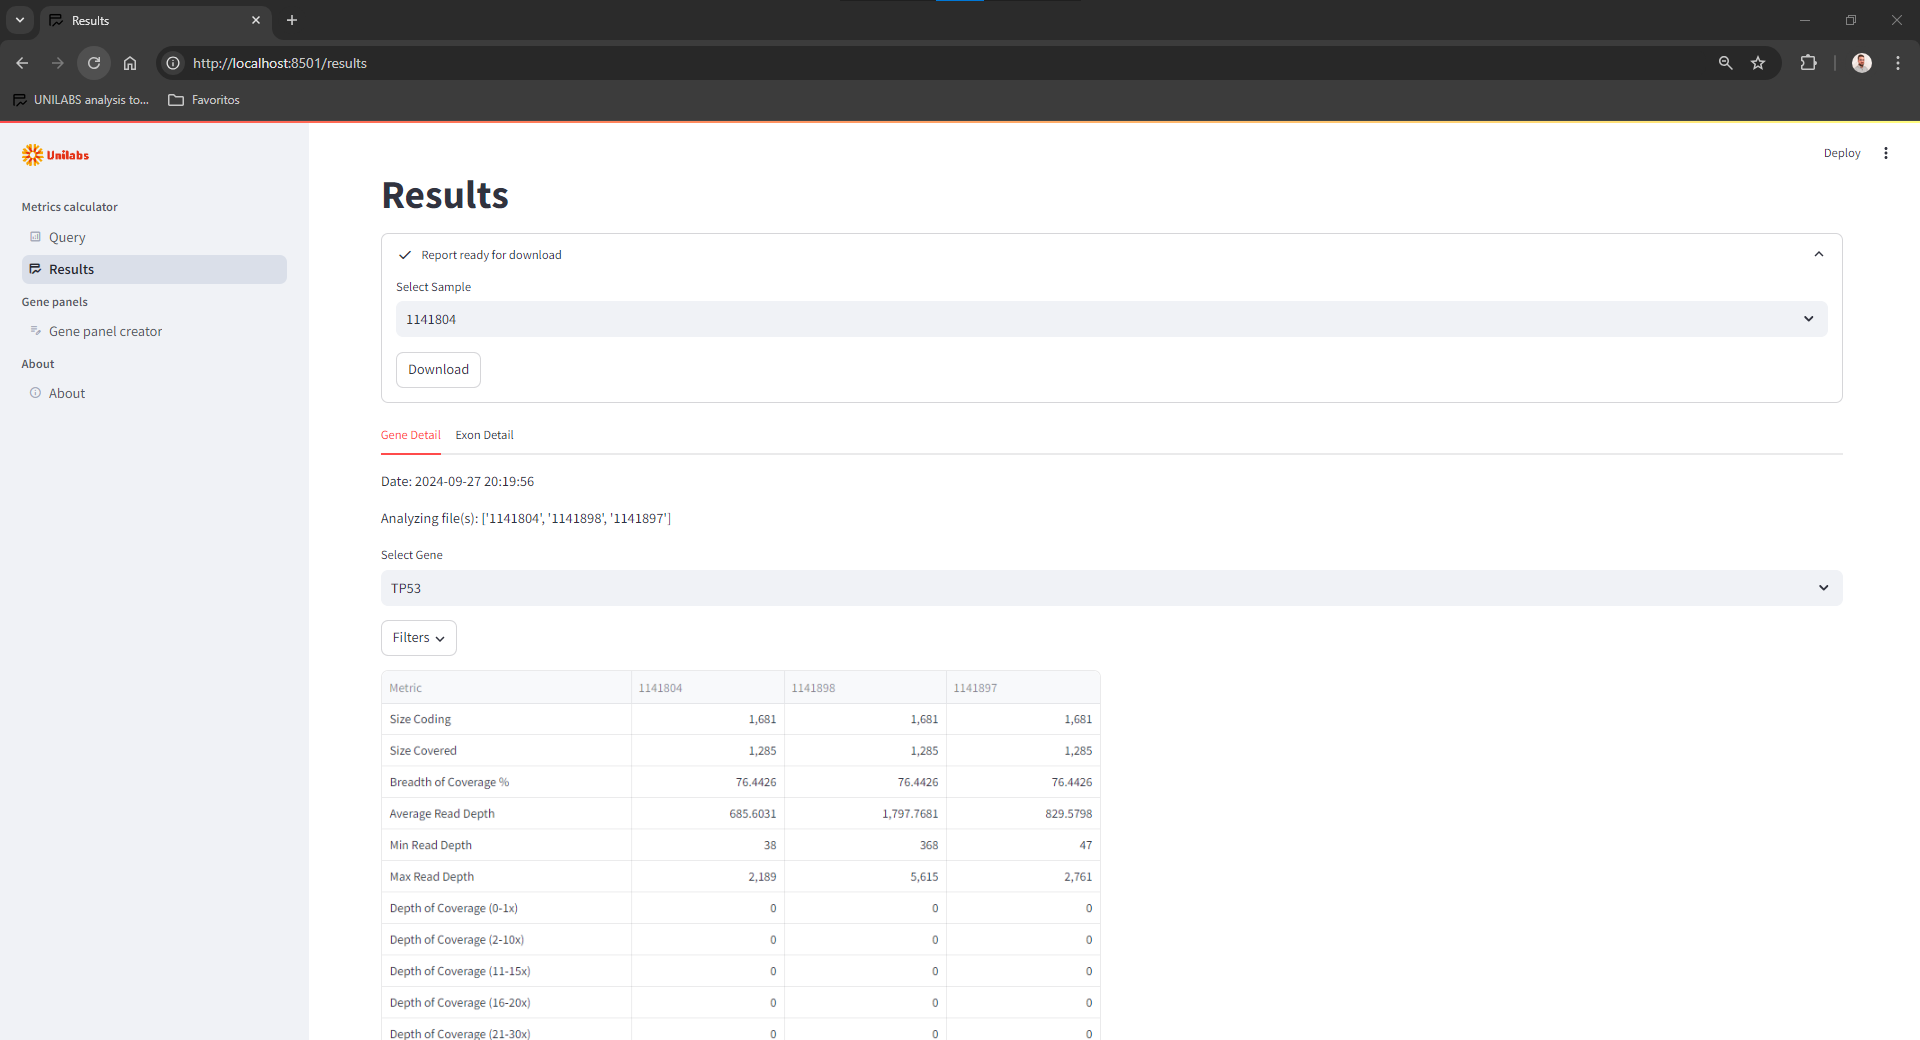
\includegraphics[width=\textwidth]{figs/v3.3.png}
        \caption{Results Tab Loading the Final Report}
        \label{fig:results_loading}
    \end{figure}
    
    In Figure \ref{fig:results_loading} and \ref{fig:final_report}, the detailed metrics for the gene \textit{TP53} are displayed, offering both gene-level and exon-level statistics. This comprehensive breakdown allows researchers to thoroughly assess the sequencing coverage for the analyzed samples. Key metrics include the size coding of the gene, minimum and maximum read depth, and coverage percentages across various depth thresholds, providing valuable insights into the quality and completeness of the sequencing data.
    
    For this case study, the size coding of the \textit{TP53} gene is 1,681 base pairs (bp), with a covered size of 1,285 bp for all three samples, resulting in a Breadth of Coverage of 76.4\%. The average read depth across the three samples was 685.6x, 1,797.8x, and 829.6x, respectively. Sequencing depth, or the number of times a particular region of the genome is covered by reads, directly impacts the reliability of variant detection, gene expression studies, and other genomic analyses. Inconsistent or insufficient depth may lead to variability in the ability to accurately detect mutations or copy number variations, potentially resulting in false positives or false negatives. For instance, lower depth may miss variants that are present at low frequencies, while higher depth ensures that even rare mutations are confidently identified. \cite{Larson2023}
    
    When examining the depth of coverage across different thresholds, the coverage percentages for the 10x, 20x, and 30x thresholds were consistently 100\% for all three samples, demonstrating that all regions of interest achieved sufficient coverage at these lower thresholds. However, at higher thresholds, the depth of coverage showed more variability. For the 50x threshold, the coverage percentages were 95.3\%, 100\%, and 99.2\%, respectively. Similarly, at the 100x threshold, the coverage percentages were 83.8\%, 100\%, and 78.5\%. Finally, at the highest threshold of 500x, the coverage percentages dropped more significantly, with values of 41.4\%, 88.2\%, and 52.8\%, respectively.
    
    \begin{figure}[H]
        \centering
        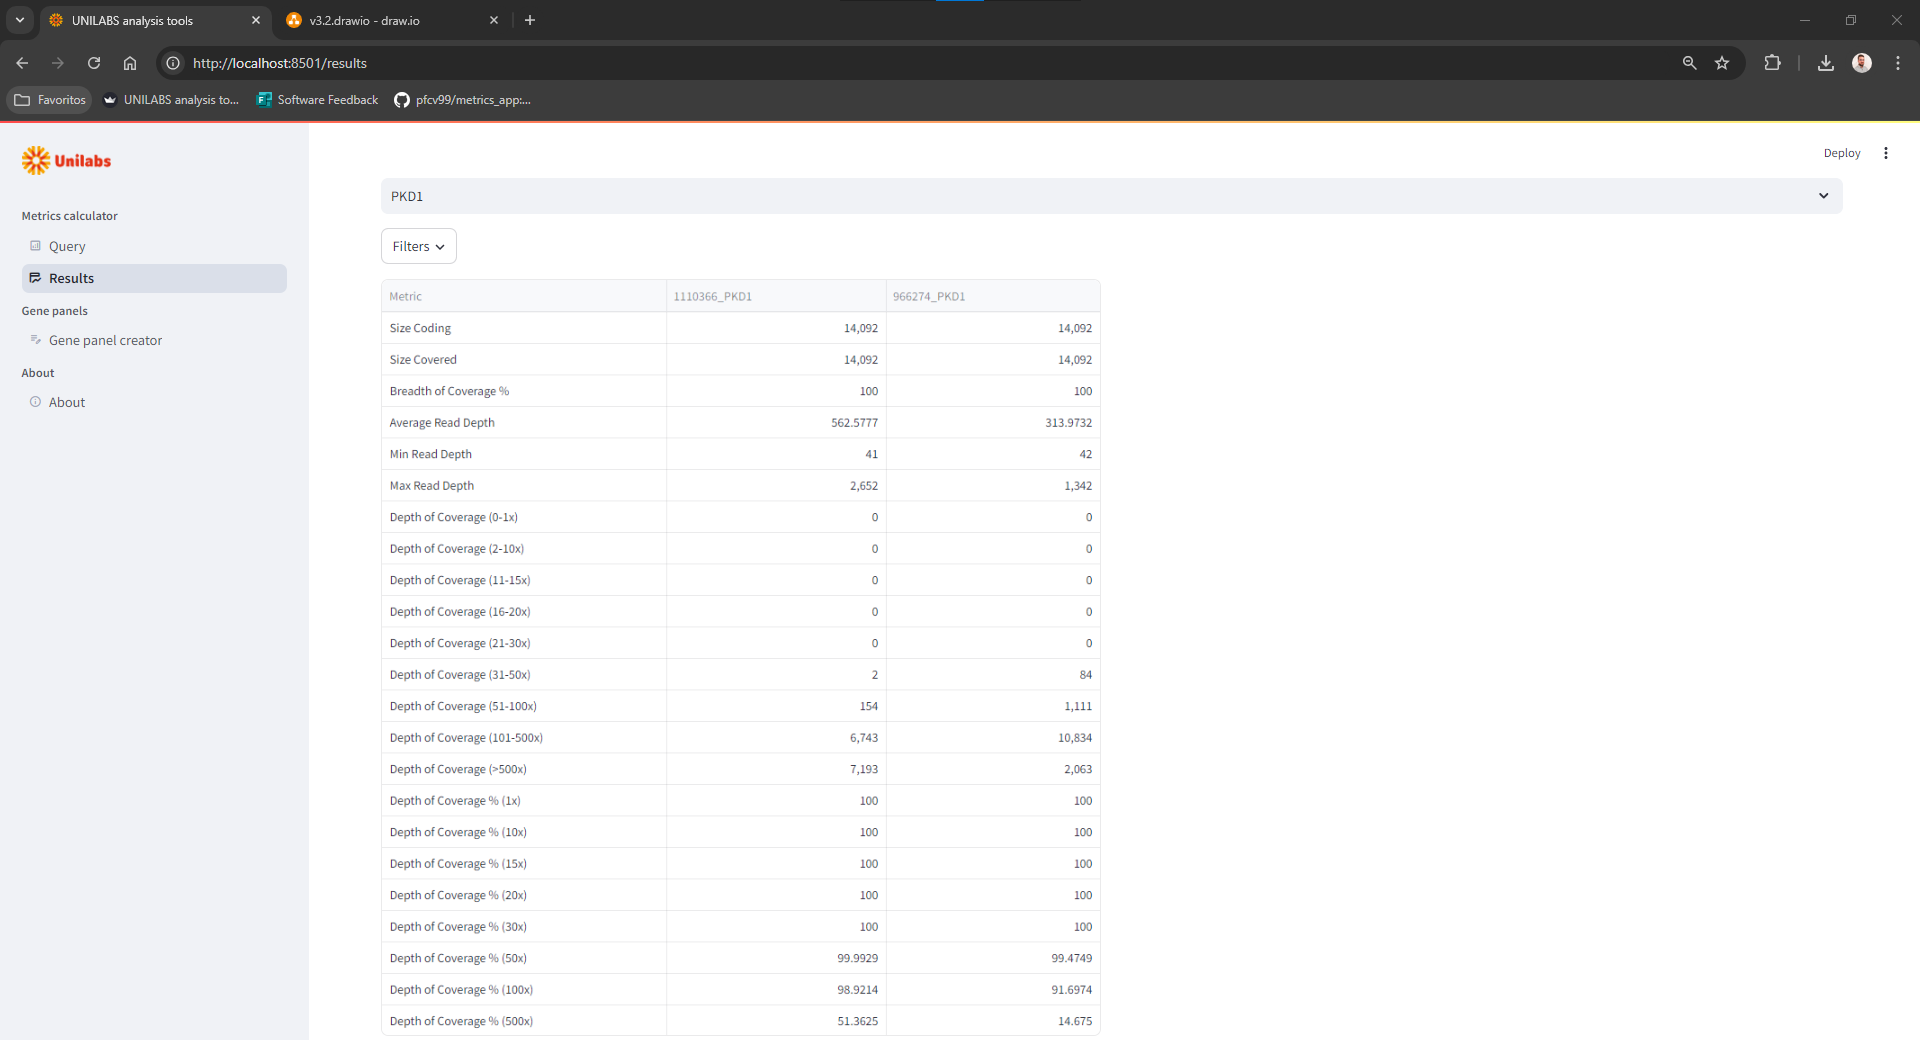
\includegraphics[width=\textwidth]{figs/v3.4.png}
        \caption{Final Report with Detailed Metrics for Gene TP53}
        \label{fig:final_report}
    \end{figure}
    
    \item \textbf{Depth of Coverage Visualization}
    
    One of the critical features of the final software version is its ability to visualize depth of coverage, as shown in Figure~\ref{fig:coverage_plot}. This visualization allows users to see the depth of sequencing across the gene of interest, with blue regions highlighting exons. A threshold can be set by the user, and regions that fall below this threshold are highlighted in red, ensuring that gaps or low-coverage areas are easily identified. This is particularly important for researchers assessing the completeness of their sequencing data.
    
    \begin{figure}[H]
        \centering
        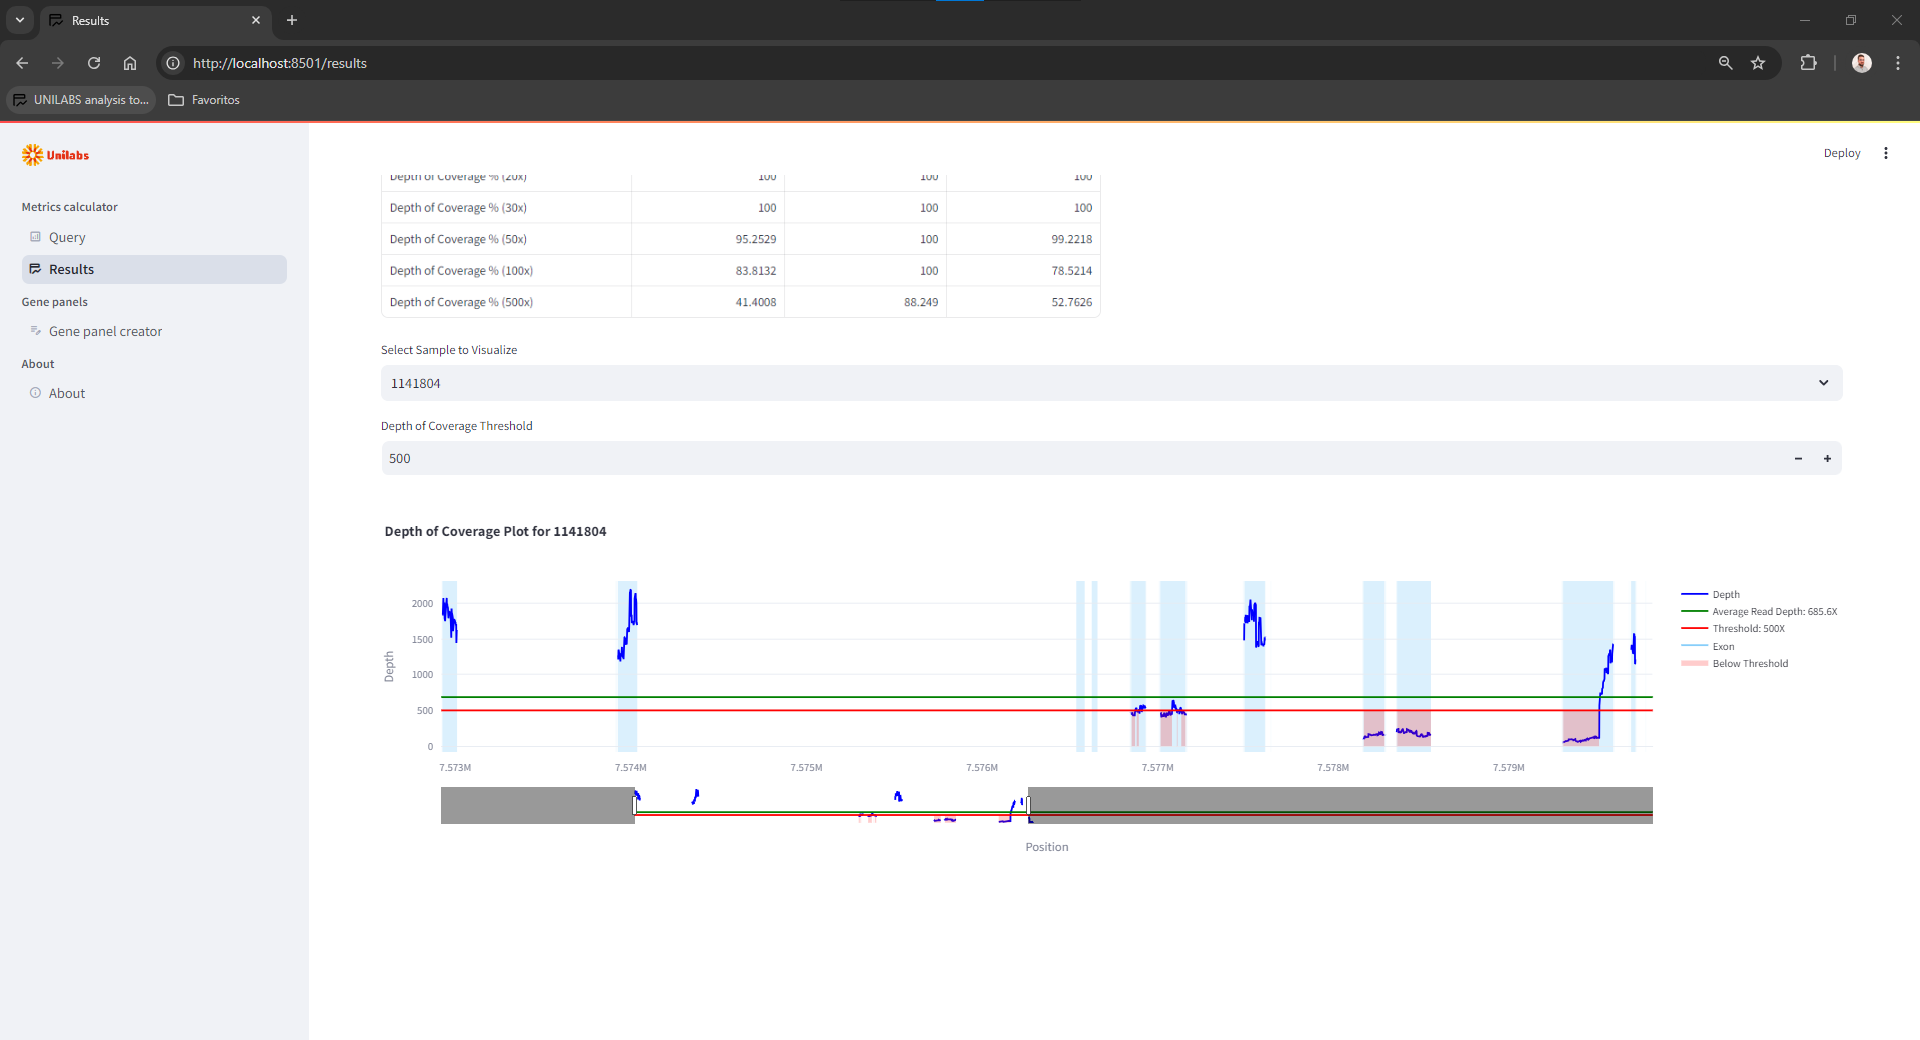
\includegraphics[width=\textwidth]{figs/v3.5.png}
        \caption{Depth of Coverage Visualization for Gene TP53}
        \label{fig:coverage_plot}
    \end{figure}
\end{itemize}

\subsubsection{\textbf{Gene Panel Analysis}}



\section{Test and validation}

De forma a validar a ferramenta, foram realizados testes com dados reais de sequenciação genómica. Os resultados obtidos foram comparados com os obtidos por outras ferramentas de análise de dados genómicos comerciais, como a \textit{Omnomics}. Foram reproduzidas as análises para Singles Gene e Gene Panel. 
No primeiro caso, para o mesmo ficheiro de alinhamento .bam, e usando como referência a mesma versaão do genoma humano (hg19), os resultados obtidos foram semelhantes como se pode observar na Figura

\section{Performance}


\section{Comparison with other tools}


\section{Users feedback}






